\chapter{Introduction, Theory, and Background}

%\textcolor{blue}{I have a lot of different important concepts that I need to 
%get through, so I can easily imagine this becoming a relatively long 
%introduction compared to other master's theses.}

A primary goal of cosmology is to specify, as narrowly as possible, the 
parameters that define our Universe. These include, for example, the overall 
curvature of the Universe as well as its cold dark matter (CDM) content. The 
evolution of the Universe depends on its contents. For example, when the 
proportion of matter is high enough,
gravity will cause the Universe to collapse again on itself. By contrast, if
the proportion of dark energy is high enough, the Universe will continue to
accelerate in its expansion forever.

Cosmology has rapidly evolved into a high-precision science. The cosmic
microwave background (CMB) is the most powerful cosmological probe and
several. With
COBE (1989-1993) \cbib{COBE} followed by WMAP (2001-2010) \cbib{WMAP} followed 
by Planck (2009-2013) \cbib{Planck}, the uncertainties on several cosmological 
parameters have been tightened significantly.
Galaxy clustering is another important probe, with similarly ambitious
improvements over the years. The original Sloan Digital Sky Surveys (SDSS) I
and II covered about one million galaxies in a redshift range of $0.07 < 0.2$
and were completed over the periods 2000-2005 and 2005-2008, respectively.
The Dark Energy Spectroscopic Instrument, which had its first light in 2019, is expected to complete its mission of 30 million targets in 2026.
\cbib{Finkbeiner}. These probes allow us to describe the matter power spectrum
with greater precision. The power spectrum is the amplitude of density
fluctuations as a function of scale. It is therefore a representation of how
matter clustering depends on physical separation.

The CMB and galaxy clustering probes have been crucial to the establishment
of the $\Lambda$CDM model as the standard model of cosmology. Under this
model, the Universe is dominated by a dark energy component in the form of a
cosmological constant $\Lambda$, which behaves like a vacuum energy constant
in density across space and time. This model also posits a dark matter
component which is ``cold'' (meaning a negligible velocity dispersion and
therefore a negligible pressure) and constitutes the vast majority of matter
in the Universe.

There are several related mysteries about the Universe that we would like to
explore, such as the nature of dark energy and the origin of primordial
fluctuations. These mysteries can be explored by testing our observations
against several extensions of the $\Lambda$CDM model, such as a nonzero 
curvature component or a time-dependent dark energy equation of state. 

Statistical analyses to answer these questions rely on great numbers of
evaluations of cosmological theory in order to build probability 
distributions, from which we obtain estimates for parameters and their
uncertainties. These evaluations of cosmological theory entail the solutions
of computationally-expensive equations (see
section~\ref{sec: boltzmann_intro}). The time spent on these evaluations
represents a bottleneck of the analysis which can be alleviated by the
use of an emulator, a kind of multi-dimensional interpolator.

After training an emulator over many theory evaluations, we can use the
emulator instead of continuing to solve the equations. Furthermore, in
a technique known as \textit{evolution mapping}
(section~\ref{sec: ev_mapping_intro}), we can exploit a degeneracy between 
several parameters and dramatically reduce the number of parameters over which
we need to train. 

In summary, the goal of this work is to extend the applicability of
evolution-mapping emulators to cosmologies with massive neutrinos by
including a parameter otherwise behaving as a degenerate parameter. 

\section{Brief Glossary of Our Cosmological Parameters}
\label{sec: param_glossary}

We will get more specific about terms like ``cosmological observations''
and ``what we would expect to see'' in the next section (\ref{sec: Pk_intro}, 
on the matter power spectrum). First, we will briefly introduce concrete
examples of cosmological parameters in which we are interested.

In this work, we will concentrate on different parameters to different 
extents. 
% The six parameters over which our emulator is trained are
% $\omega_b$, $\omega_c$, $n_s$, $\sigma_{12}$, $A_s$, and $\omega_\nu$.
By the end of this thesis, we will have built and tested two main
emulators, each of which is trained over a different parameter
space.\footnote{Emulators will be described in greater detail in
section~\ref{sec: emulation_intro}. For now, the extremely simple definition 
from the summary will suffice.}
Each emulator accepts as $\matr{X}$ arrays of tuples of values for 
cosmological 
parameters and predicts as $\hat{\matr{Y}}$ the power spectra to which these
tuples correspond. 

%s Introduce the parameter names, THEN talk about what they mean

The primary emulator for this work has been trained over six parameters:
$\omega_b$, $\omega_\text{CDM}$, $n_s$, $\sigma_{12}$, $A_s$ and $\omega_\nu$.
A secondary, ``support'' emulator has been trained over just the first four of
these. The terms $h$ and $z$ are not subject to emulation but will be 
important to the generation of training data for the emulator (see 
section~\ref{sec: train_emu}. Cosmological terms beyond these (such as
$\Omega_k$, $\omega_\text{DE}$, $w_0$, $w_a$) make only minor appearances in 
this work.

%s First: introduce equations until we can explain h and omega_i

Our first goal will be to define the various $\omega_i$ terms, although along
the way it will be convenient to point out other terms. To arrive at
definitions for $\omega_i$, we will begin with the concept of the Universe's 
energy density $\rho_i$
in some energy species associated with the label $i$. We list the various
energy species and their corresponding labels in
table~\ref{tab: species_symbols}.
We note that $\gamma$ does not play a role in this thesis;
while radiation is critically important in the early stages of the
Universe, it rapidly becomes inconsequential; after the Universe was a mere
55,000 years old, the
era of radiation domination gave way to the era of matter domination 
(\cbib{CO}, page 1194)\footnote{For those who are
curious, $\omega_\gamma$ ends up being a shape parameter \cbib{FECS}.}.

%s What do the subscripts mean?

\begin{table}[htb]
\centering
\begin{tabular}{l|l}
\hline
Symbol & Energy Species \\ \hline
$\gamma$ & Relativistic (i.e. radiation, photons) \\
$B$ or $b$ & Baryons \\
$C$, $c$, or CDM & Cold dark matter \\
$\nu$ & Neutrinos \\
$M$ & Matter ($b$, CDM, and $\nu$ together) \\
DE & Dark Energy \\
$\Lambda$ & Cosmological constant (one proposal for DE) \\
$K$, $k$, or $\kappa$ & Curvature \\ \hline
\end{tabular}
 \caption[Energy species symbols]{The various energy species into which the 
 	contents of the Universe are categorized, and their conventional symbols.}
 \label{tab: species_symbols}
\end{table}

% Now that we have explained the meaning of the $\omega_i$ term in general, we
% can discuss the different specific species of energy and the subscripts that
% we use to denote them.

These densities $\rho_i$ are frequently rewritten with the help of various 
constants and cosmological parameters. We rewrite the $\rho_i$ terms are based 
on their appearance
in the equations that govern the evolution of the Universe. This discussion
will very closely follow section 2.2 from \cbib{FECS}. The reader is
encouraged to engage this source in the event of confusion, as our discussion 
here will be brief and therefore assume a great deal of cosmological 
background from the reader.

One way of writing the first Friedmann equation is:

%!s This whole next section is ripped from FECS. Should I be concerned?

\begin{equation}
\label{eq: Friedmann1}
\left( \frac{\dot{a}}{a} \right)^2 = \frac{8 \pi G}{3} \, \rho - \frac{K}{a^2}
\end{equation}

Where the dimensionless scale factor $a$ is a way of describing the size of
the Universe (which, by convention, is set to unity at the present day). As 
the universe expands, the wavelength of traveling light is stretched out, and
photons lose energy. As far as we understand cosmology today, the Universe has
always been expanding (although the expansion rate has evolved).
Therefore,\footnote{\textcolor{red}{Actually, equation~\ref{eq: a_to_z}}
should hold regardless of that fact, right? So this ``therefore'' is wrong,
right?} we
can use cosmological redshift $z$ as a proxy for the age of the Universe at 
which any photon, which we receive, was emitted from the source we are 
observing.\footnote{Photons can of course be redshifted also according to the
Doppler shift (the motion of bodies along the line-of-sight of the 
observation). On the scale of cosmological observations, cosmological redshift
certainly dominates, but distortions due to Doppler-shifted light,
called redshift space distortions, can cause problems for cosmological 
analyses. These problems lie outside the scope of this work. For a detailed
treatment on RSD, see chapter 8 of \cbib{FECS}}. Specifically, the redshift of
incoming light can
be related to the scale factor at the time of its emission as:

\begin{equation}
\label{eq: a_to_z}
a = \frac{1}{1 + z}
\end{equation}

\textcolor{red}{Is it really important that I produce some sketch to show the
effect of cosmological expansion on light wavelenghth, for example? I don't
want to waste time learning InkScape.}

$K$ characterizes the Universe's curvature as

\begin{equation}
^{(3)}R = \frac{6K}{a^2}
\end{equation}

\textcolor{red}{where $R$ is the scalar of curvature. How are we indexing
into a scalar??.}

All the energy species that make up the Universe can be approximated as
barotropic fluids with a constant of proportionality $w$ between the
pressure $p$ and the density $\rho$ of the fluid, i.e. $p = w \rho$. $w$ is
referred to as the equation of state parameter and in most cases is a
well-known constant (for example, $w_\gamma = 1/3$ and $w_m = 0$). However, in
the case of dark energy, the constancy cannot be taken for granted and we
adopt a more general form called the Chevallier-Polarski-Linder (CPL) 
parameterization \cbib{Scherrer}:

\begin{equation}
w_\text{DE} = w_0 + w_a (1 - a)
\end{equation}

These $w_0$ and $w_a$ are cosmological parameters which also appear in our
statistical analyses, although our observations so far appear to support
a cosmological constant solution: $w_0 = -1$ and $w_a$ = 0.

We can combine the equations of state for the barotropic fluids with energy 
conservation (\textcolor{orange}{Look up a derivation}) to find that

\begin{equation}
\rho_i \propto a^{-3 (1 + w_i)}
\end{equation}

As long as the different energy species do not interact, this relation will
apply to each species separately, and we can sum over all species to write:

\begin{equation}
\rho = \sum_i \frac{\rho_{i, 0}}{a^{3(1 + w_i)}}
\end{equation}

where the nought indicates the value today.

We can combine this with \ref{eq: Friedmann1} to write:

\begin{equation}
\label{eq: Friedmann1_sum}
\left( \frac{\dot{a}}{a} \right)^2
=
\frac{8 \pi G}{3} \, \sum_i \frac{\rho_{i, 0}}{a^{3(1 + w_i)}} - \frac{K}{a^2}
\end{equation}

%s Introduce h

At this point, we have tied in all of the physics that will be necessary to
explain the $\omega$ and $h$ parameters--now it is just a matter of rewriting 
terms. First, we define the \textit{Hubble parameter}
$H \equiv \frac{\dot{a}}{a}$ and evaluate \ref{eq: Friedmann1_sum}
for the present:

\begin{equation}
\label{eq: Friedmann1_present}
H_0^2 = \frac{8 \pi G}{3} \, \sum_i \rho_{i, 0} - K
\end{equation}

$H$ is customarily written in units of
$\frac{\mathrm{km}}{\mathrm{s} \mathrm{Mpc}}$, and the constant
$H_{100} = 100 \, \frac{\mathrm{km}}{\mathrm{s} \mathrm{Mpc}}$ can be used to
define the \textit{dimensionless Hubble parameter} $h = \frac{H_0}{H_{100}}$.

%\textcolor{red}{Why do we bother with $H_{100}$ at all? Why didn't we just
%define }

In terms of $h$, equation \ref{eq: Friedmann1_present} becomes

\begin{equation}
h^2 = \frac{8 \pi G}{3 H_{100}^2} \, \sum_i \rho_{i, 0} - \frac{K}{H^2_{100}}
\end{equation}

%s Introduce \omega and \Omega  

Since the coefficient has units of density, it is convenient to define the
dimensionless \textit{physical density parameters}

\begin{equation}
\omega_i \equiv \frac{8 \pi G}{3 H_{100}^2} \rho_{i, 0}
\end{equation}

The analog for curvature is defined separately as

\begin{equation}
\omega_{K} \equiv -\frac{K}{H_{100}^2}
\end{equation}

The dimensionless physical density parameters are traditionally bypassed in
favor of the \textit{fractional density parameters} $\Omega_i$:

\begin{equation}
\Omega_i \equiv \frac{\omega_i}{h^2}
\end{equation} % = \frac{\rho_{i, 0}}{\rho_c}

which has the conceptual advantage of summing to unity when the Universe is
flat. However, the inclusion of $h^2$ in the definitions of the density
parameters can lead to misconceptions which are relevant to the content of
this work but are beyond its scope. The simplest argument against the use of 
$\Omega_i$ for the purposes of
this treatment is that $\Omega_i$ combines two unknowns, $h$ and $\rho_i$
together, which complicates parameter inference.\footnote{This situation is 
made more drastic due to the Hubble tension, which leaves the value of $h$ 
fairly unclear compared to other parameters.} Therefore, for this work we
will use $\omega_i$ instead.

%s Distinguish baryons from CDM

While baryons and cold dark matter (CDM) are both pressureless\footnote{This 
is of
course an approximation, but it is a very good one. While a hot baryonic gas 
certainly exerts a pressure, this pressure is negligible in comparison to the energy density of the gas. \textcolor{red}{Where are we getting a unitless
pressure term such that we can compare it in this way to energy density?
Otherwise, terms of different units cannot be compared. I understand that we
can get a unitless energy density by making it relative. Is there a similar
procedure for pressure terms?}}, CDM appears to interact only gravitationally
with other matter. This lack of collisional and radiative self-interaction
prevents CDM clouds from collapsing in the same way that, for example,
baryons can collapse to form stars and planets. Because of the significantly
different behaviors of these two species of matter, we treat them separately
even in cosmological contexts.

%s omega_k

\textcolor{red}{According to Andrea P., $\omega_K$ is an evolution parameter 
only in a narrow 
band around zero--specifically, over roughly the range [-0.05, 0.05].
By how much does evolution mapping fail here? And, if 
$\omega_K$ is truly a shape parameter, why does Ariel's FECS call $\omega_K$
an evolution parameter?} We do not emulate over $\omega_K$ but assume take
it to be zero for all cells. However, as we explain in
section~\ref{sec: ev_mapping_intro}, this does not limit the applicability of
our emulators. The use of nonzero $\omega_K$ values will simply entail a
relabeling of the emulated power spectra. \textcolor{orange}{Then again, I'm
holding $\sigma_{12}$ fixed, so does it change anything at all?}

%s n_s

The parameter $n_s$ is called the \textit{spectral index} and describes the 
power laws
to which the power spectrum may be fit. We will delay its explanation to
section~\ref{sec: Pk_intro}, where we introduce the power spectrum.

%s A_s

The parameter $A_s$ is called the \textit{scalar mode amplitude} and describes
the amplitude of the primordial power spectrum. We will explore the subtlety of this parameter's impact in
chapter~\ref{chap: A_s}.

%s sigma12 versus sigma8. This should come last as it is by far the most
%s challenging of the parameters to explain.

To conclude this section, we will briefly introduce the parameter
$\sigma_{12}$, which will be fleshed out in
section~\ref{sec: boltzmann_intro}. 
$\sigma_{12}$ is defined as the linear-theory RMS mass variance in spheres
of radius 12 Mpc:

\begin{equation}
\label{eq: sigma12}
\sigma_{12}
=
\sqrt{\left\langle \left(
	\frac{\delta M}{M} (12 \, \mathrm{Mpc})
\right)^2 \right\rangle}
\end{equation}

As with the $\omega_i$ parameters, there is a more conventional parameter
which again relies on the dimensionless Hubble parameter. $\sigma_8$ is
defined as

\begin{equation}
\sigma_8
=
\sqrt{\left\langle \left(
	\frac{\delta M}{M} (8 \, \mathrm{Mpc} \, h^{-1})
\right)^2 \right\rangle}
\end{equation}

Notice that this is \textit{not} the same as replacing 12 with 8 in
equation~\ref{eq: sigma12}! The subscript in $\sigma_8$ is misleading:
$\sigma_8$ is the linear-theory RMS mass variance in spheres of radius
$8 / h$ Mpc, not 8 Mpc. Recall that $h$ is not a well-known constant but its 
own  cosmological parameter whose value is subject to further observations.

$h$ units (which will appear again in section~\ref{sec: Pk_intro}) became
conventional with the first galaxy redshift surveys (GRSs). The conversion of
redshifts into comoving distances $\chi(z)$ requires the assumption of a set 
of
cosmological parameters called a \textit{fiducial cosmology}. However, the
earliest surveys probed a limited range of small redshifts, where the
comoving distance may be estimated as follows:

\begin{equation}
\label{eq: comov_dist_approx}
\chi(z) \approx \frac{c}{H_0} \, z
\end{equation}

Therefore, use of $h^{-1}$ Mpc units allowed analyses of these early GRSs
to quote results without assuming a fiducial cosmology. This
approximation loses its validity for later GRSs because they covered larger
redshift ranges. Without this approximation then, the analyses of these later
surveys had to assume a full fiducial cosmology anyway. This means that
$h^{-1}$ Mpc units lack their original justification, although out of
convention they continue to be used (\cbib{San20}).

This convention is not without serious drawbacks.
For example, our incomplete understanding of $h$
becomes problematic when comparing the results of different papers;
if the quoted $h$ values differ even slightly between two works, the same
symbol $\sigma_8$ will refer to different concepts--that is, mass variances on
different scales. Therefore $\sigma_8$ comparisons will typically lead to
confusion, such as the $\sigma_8$ tension, which basically vanishes when using
$\sigma_{12}$. For a fuller treatment of the advantages of $\sigma_{12}$, we
refer the reader to \cbib{San20}.

The issue with $\sigma_8$ most relevant to this work is that, like the
fractional density parameters $\Omega_i$, $\sigma_8$ combines two uncertain
cosmological quantities: the amplitude of the power spectrum, and the
relative expansion rate of the Universe. Even more important is the evolution 
mapping argument. We can greatly simplify the
parameter space of emulators with the help of $\sigma_{12}$
(see section~\ref{sec: ev_mapping_intro} for details), and $\sigma_8$
is simply incapable of exploiting the parameter degeneracies in the same way.


\section{The Matter Power Spectrum}
\label{sec: Pk_intro}

Now that we have at least briefly introduced the various cosmological
parameters of interest to us, we can define what we meant in the opening
paragraphs by ``cosmological observations'' and ``what we would expect to
see.'' How can we describe the Universe in such a way as to allow quantitative 
definitions of these phrases? As a starting point, we can imagine quantifying 
the energy density $\rho(\bm{x})$ of the Universe at any one point $\bm{x}$ in 
three-dimensional space.

%Let us return to the idea that cosmological parameters determine the the 
%evolution of the Universe.
% In what ways can we quantify the Universe, in order to be able to describe
% its evolution? We can simply consider the time dependence of the density.

We can define a similar quantity, a relative density:

\begin{equation}
\delta(\bm{x}) = \frac{\rho(\bm{x}) - \bar{\rho}}{\bar{\rho}}
\end{equation}

which we refer to as the ``matter density contrast field.'' $\bar{\rho}$
represents the average energy density of the entire Universe. 
$\delta(\bm{x})$ easier than $\rho(\bm{x})$ to work with since it
is unitless and especially because it is normalized--the integral of the
matter density contrast field, taken over the entire Universe, is unity.

$\delta(\bm{x})$ may in turn be used to define the two-point correlation 
function:

\begin{equation}
\xi(\bm{r})
=
\langle \delta (\mathbf{x}) \delta(\mathbf{x} + \mathbf{r})\rangle
\end{equation}

This may be rewritten as $\xi(r)$ (i.e., the separation vector becomes a
separation scalar) by application of the cosmological principle: on large
enough scales ($r \gtrsim 100$ Mpc) \, the Universe looks statistically 
homogeneous and isotropic (\cbib{Ntelis}). That is, there are neither 
preferred regions nor directions, but rather all parts of the Universe are
indistinguishable.

Unlike $\delta(\bm{x})$, $\xi(r)$ follows from our cosmological
observations. Consider a basic GRS scenario: the
measured redshift acts as a proxy for the line-of-sight distance (subject to
the application of some fiducial model) between the observer and the galaxy. 
By combining this distance with the sky position (the two angles $\theta$ and
$\phi$), we can locate each galaxy in three-dimensional space. Then, $\xi(r)$ 
may be estimated via analysis of every pair of galaxies in our data. Simply
put, within such a survey, $\xi(r)$\footnote{Technically, this is a statement
about $\xi_g(r)$, the two-point correlation function of galaxies. Although we
are using galaxies to approximate the distribution of all matter, there will
be some bias in our approach because galaxies (as extraordinarily dense 
structures) represent peaks in the $\delta$ field.} can be thought
of as the excess probability that some galaxy will be located at a distance
$r$ from any other galaxy.

Lastly, to arrive at the object of primary interest to this work, we will
consider the Fourier transform of $\xi(r)$, which gives us the power spectrum:

\begin{equation}
P(k) = \int d^3 r \, \xi(r) \exp [i \bm{r} \cdot \bm{k}]
\end{equation}

%s Why isn't this project obsolete, what with nonlinear emulators?

The power spectrum describes the variance of the amplitudes of the Fourier
modes. Actually, the power spectra we are discussing in this thesis are 
\textit{linear-theory} power spectra $P_\text{L}(k)$ of \textit{non-neutrino} 
matter.\footnote{\textcolor{red}{Andrea added the following comment: ``We 
should 
justify this assumption. It is standard practice to assume that the galaxy 
density field is determined only by the underlying cdm+b density field, 
without taking into consideration the cold neutrino component (which also 
behaves as matter).'' Do you have recommendations for sources I can consult in
order to add this information to this paragraph?}} Emulators of non-linear 
power spectra $P_\text{NL}(k)$ are 
already available, but linear-theory power spectra are still important.
For example, they can be used to predict $P_\text{NL}(k)$, like in 
perturbation theory approaches. Furthermore, most non-linear emulators
actually predict the ratio of the non-linear power spectrum to its linear
counterpart, so $P_\text{L}(k)$ is still necessary to evaluate
$P_\text{NL}(k)$ (A. G. S\'{a}nchez, private communication, 2022).

Matter density fluctuations grow at different rates depending on 
the dominant energy species in the Universe, and so far the Universe has
undergone two major periods of domination (only relatively
recently have we entered a third period, dominated by dark energy): first by 
radiation, then by matter. The power spectrum captures this history. The
smaller Fourier modes, which entered the \textit{comoving particle horizon} 
(maximum
separation of two particles in causal contact) $\chi_h$ first, were strongly
suppressed by radiation, with

\begin{equation}
\chi_h = \int_0^{t_0} \, \frac{dt}{a(t)}
\end{equation}

By contrast, the larger Fourier modes, which
entered the horizon during matter domination, more easily grew in structure
(\cbib{Dodelson}). The power spectrum can be fit by a piecewise function of 
two parts, depending on when a Fourier mode enters the horizon.
During the matter-dominated era, 

\begin{equation}
\label{eq: n_s}
P(k) \propto 
\begin{cases}
      k^{n_s} & k \ll k_\text{eq} \\
      k^{n_s - 4} [\ln (k)]^2 & k \gg k_\text{eq} \\ 
    \end{cases}\,.
\end{equation}

Where $n_s$ is the spectral index mentioned in
section~\ref{sec: param_glossary} and

\begin{equation}
\label{eq: turnover}
k_\text{eq} = 0.073 \, \omega_m \, \mathrm{Mpc}^{-1}
\end{equation}

is called the turn-over scale \cbib{FECS}.

%s Why do we care about the power spectrum?

So, already from these two equations, we can
appreciate that the power spectrum helps us to constrain two key cosmological
parameters: $n_s$ and $\omega_m$. It turns out that the precise shape and
amplitude of the power spectrum can tell us about all of the six primary
parameters that we introduced in section~\ref{sec: param_glossary}:
$\omega_b$, $\omega_c$, $n_s$, $\sigma_{12}$, $A_s$, and $\omega_\nu$. 
Specifically, the power spectrum is useful for parameter inference because of
its \textit{unique} dependence on each of these parameters. In 
section~\ref{sec: boltzmann_intro}, we will include several figures 
illustrating more clearly what these different dependencies look like.

%s Now show a picture

\begin{figure}[htb]
  \centering
  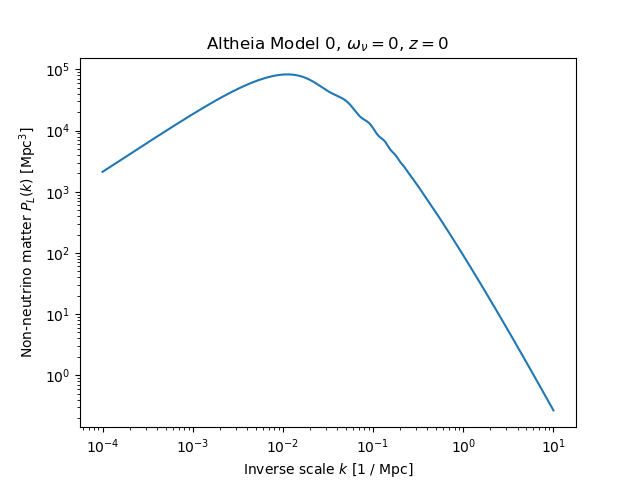
\includegraphics[scale=1.0]{intro/m0_Pk}
  \caption[Aletheia Model 0 Power Spectrum]{This is power spectrum was
  computed by CAMB for Aletheia model 0 without massive neutrinos.
  Table~\ref{tab: Aletheia_m0} defines this model in terms
  of the parameters essential to this work.}
  \label{fig: first_power_spectrum}
\end{figure}

\begin{table}[htb]
\centering
\begin{tabular}{l|l}
\hline
Parameter & Value \\ \hline
$\omega_b$ & 0.022445 \\
$\omega_c$ & 0.120567 \\
$n_s$ & 0.96 \\
$\sigma_{12}$ & 0.82476153 \\
$A_s$ & $2.1272 \cdot 10^{-9}$ \\ \hline
\end{tabular}
 \caption[Aletheia Model 0 Parameters]{This table describes
 figure~\ref{fig: first_power_spectrum} in terms of the parameters
 essential to this work. $A_s$ is truncated to five significant figures.
 Model 0 is a helpful benchmark model because it uses
 best-fit values from the Planck CMB measurements. Aletheia model 0 does not
 itself specify a physical density in neutrinos, but we will typically use
 $\omega_\nu = 0$. Unlike the rest of model 0, this setting is strongly 
 	discounted by our current cosmological observations.}
 \label{tab: Aletheia_m0}
\end{table}

A standard Planck $\Lambda$CDM model is shown in
figure~\ref{fig: first_power_spectrum}. The turnover scale $k_\text{eq}$
(eq~\ref{eq: turnover}) marks
the transition between the radiation- and matter-dominated epochs, as
$k_\text{eq}$ is the first (and therefore) smallest Fourier mode to enter the 
comoving particle horizon $\chi_h$ during the era of matter domination, where

\begin{equation}
\chi_h = \int_0^{t_0} \, \frac{dt}{a(t)}
\end{equation}

Figure~\ref{fig: first_power_spectrum} also shows the baryon acoustic
oscillation (BAO) as a set of shallow wiggles on inverse scales of roughly
$0.04 < k \, \text{Mpc} < 0.2$. The BAO is beyond the scope of this paper but,
briefly put, is the signature of a shock wave generated during the epoch of
radiation domination before baryons decoupled from photons. As baryons
collapsed into dark matter gravitational potential wells, the radiation
pressure eventually became high enough to reverse the collapse.

%s Everyone else uses h units. Why don't we?

Experienced readers will notice that our power spectrum in
figure~\ref{fig: first_power_spectrum} does not use the customary $h$ units:
our $x$-axis uses units of Mpc$^{-1}$ rather than $h$ Mpc$^{-1}$ and our
$y$-axis uses units of Mpc$^3$ rather than Mpc$^3 \, h^{-3}$. This is yet
another instance of customary factors of $h$ (see also the $\Omega_i$ and
$\sigma_8$ discussions in section~\ref{sec: param_glossary}). As mentioned
for $\sigma_8$, these units were introduced in the times when GRS redshift 
ranges justified the use of equation~\ref{eq: comov_dist_approx}. This
convention also persists in emulator literature (see, for example,
\cbib{Arico} and \cbib{Mancini}).

% The following plots were generated with h_units_bad.ipynb
\begin{figure}[htb]
    \begin{subfigure}{0.45 \textwidth}
    \centering
 		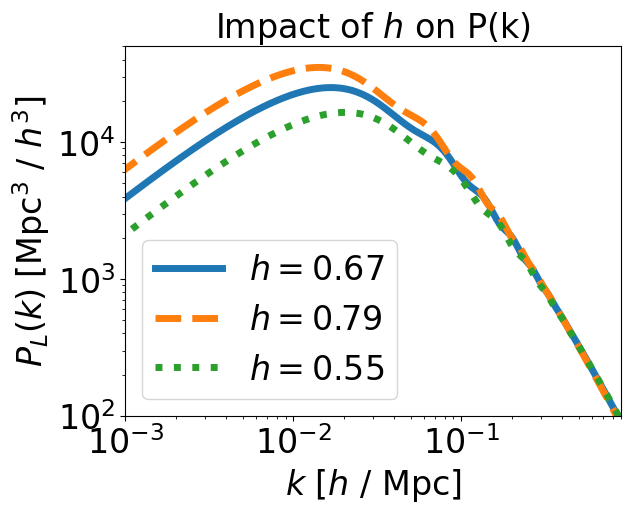
\includegraphics[width=\textwidth]{intro/h_impact_h_units}
 		\caption{Using $h$ units.}
 		\label{fig: h_units}
    \end{subfigure}
    \begin{subfigure}{0.45 \textwidth}
    \centering
 		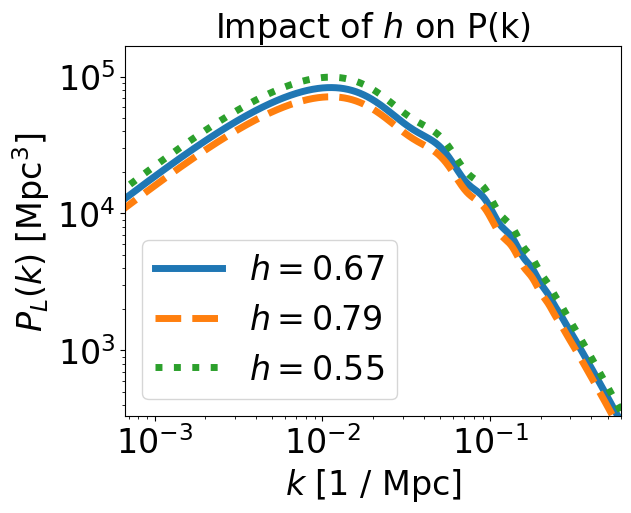
\includegraphics[width=\textwidth]{intro/h_impact_absolute_units}
 		\caption{Using absolute units.}
 		\label{fig: without_h_units}
    \end{subfigure}
        \centering
    \caption[Impact of $h$ on $P(k)$]
    		{Non-neutrino matter power spectra at $z=0$ for three different
    		models based on model zero (refer to table~\ref{tab: Aletheia_m0} 
    		for details) and varying only in the value of $h$. These two
    		panels
    		differ only in the units used. Observe that, in absolute units, we
    		can easily identify the impact of $h$ as a simple change in
    		amplitude. The use of $h$ units obscures this effect. This figure 
    		is an imitation of figure 1 from \cbib{San20}.}
    \label{fig: h_unit_Pk}
\end{figure}

%! Try to more carefully explain why it doesn't work: h is not a parameter
% over which we emulate--sigma12 is. Therefore we cannot show h in the final
% plots. This is a much subtler issue than the h complaints in the
% previous section.

Again, we refer the reader to \cbib{San20} for a detailed case against the
use of $h$ units in observational cosmology. We illustrate in
figure~\ref{fig: h_unit_Pk} one significant problem related to the
unstable meaning of $\sigma_8$: varying $h$ changes not only the power 
spectrum, but also the axes used to represent the power spectrum. Comparison 
of power spectra from different 
models is hindered because the $x$ and $y$ axes correspond to different ranges
for each curve. If we use instead units of Mpc, then changes in $h$ change
only the power spectrum, and we can much more readily appreciate its true
impact (that of an amplitude change).

As with our choice of $\sigma_{12}$ instead of $\sigma_8$, our choice of
absolute units will facilitate the application of evolution mapping described
in~\ref{sec: ev_mapping_intro}. Since $h$ only affects the amplitude of the
power spectrum, we do not need to train our emulator over it at all. Absolute 
units are not only clearer but allow us to confine all of the significance of
the value of $h$ to its impact on the value of $\sigma_{12}$.

\section{Boltzmann Solvers and CAMB}
\label{sec: boltzmann_intro}

%s What kinds of equations do we need to solve?

The power spectrum can be predicted with great accuracy via linear 
approximations. However, the evolution equations are involved (running, for
example, over many different cosmological parameters) and can be
stiff, which calls for different approaches in different regimes. Furthermore,
its solutions are highly oscillatory and therefore susceptible to numerical
errors (\cbib{Seljak}). Full solutions consist of many different steps, whose
descriptions fall outside of the scope of this work. We refer readers curious
about these equations to the history in the introduction of \cbib{Seljak},
which cites papers important to their development. 

%s Equations are hard. Who can save us?

The so-called \textit{Boltzmann codes} have been 
developed in order to leverage modern computational power and automate the
solution of these equations of evolution. Typically, Boltzmann codes offer as
outputs CMB spectra and matter power spectra. The latter is the focus of this
work.

%s What can our savior do?

As input, Boltzmann codes accept a set of values for different 
cosmological parameters, many of which were defined in section~\ref{sec: 
param_glossary}. Boltzmann codes enable us to pick from wide ranges of 
accepted values for these parameters and to consider the power 
spectrum for almost any combination of these parameters. Of course, there are 
still limitations. For example, CAMB does not currently support negative 
redshifts (which, we will later see, becomes a problem), and the minimum 
allowed value of $H_0$ is 1 km / s / Mpc, although slightly higher values have 
been observed to cause runtime errors in the presence of other extreme 
parameters.

%s Pics? Not so fast. Let's pick one.

Before we proceed to concrete demonstrations, it will be expedient to settle
on a single Boltzmann solver. As of today, the two Boltzmann codes
CAMB\footnote{\url{https://github.com/cmbant/CAMB}} and
CLASS\footnote{\url{https://lesgourg.github.io/class_public/class.html}} offer
the largest suites of features and are also actively developed. CAMB and
CLASS were written in different languages (Fortran-90 and C, respectively)
but both come with Python wrappers. These codes have been shown to be in 
excellent agreement with each other (see \cbib{Lesgourges}), and their
differences consist primarily of different approaches in algorithms (including 
speedup tricks) and user interfaces and customization options.

As the researchers in our group have much more experience with CAMB, we 
elected to use CAMB as a starting point for our Python package
Cassandra-Linear. In principal, to maximize the generality of 
the results introduced in this 
work, we would demonstrate their compatibility with at least CLASS as well. In 
practice, since these codes agree so well, we prioritize other lines of 
inquiry
for this work. However, later, in section~\ref{sec: generate_emu_data}, we 
will concede an important, 
independent reason to consider use of CLASS, which becomes a promising route
for continuation of this work (see section~\ref{sec: future_work}).

%%%
\begin{comment}
\textcolor{green}{Furthermore, the CLASS documentation
is not nearly as strong as it is with CAMB, and we already encountered
extreme difficulty simply in recreating results already previously obtained
via CAMB!}
\end{comment}
%%%

%s Examples of great results from Boltzmann solvers

To connect this section with~\ref{sec: param_glossary}, we can visualize the
impact of each of this work's core parameters on the power spectrum. One
simple way to set this up for parameter $\Theta_i$ is to designate Aletheia 
model 0 as a middle ground and to create two copies of model 0, with each
copy tweaked to have an increased or decreased value of $\Theta_i$. This
approach works for every parameter except for $\omega_\nu$, where one of the
copy cosmologies describes the middle ground since the default value
$\omega_nu = 0$ is already at a hard boundary.

When feeding these cosmologies into CAMB, our Boltzmann solver of choice, we
obtain figures~\ref{fig: omega_b_dependence}, \ref{fig: omega_c_dependence}, 
\ref{fig: n_s_dependence}, \ref{fig: A_s_dependence}, and \ref{fig: 
omega_nu_dependence}. Keep in mind that the value ranges that we have applied
here are extremely broad and have nothing to do with state-of-the-art
confidence intervals on the parameters in our Unvirse. On the 
contrary, many of the values used for these plots may be completely 
discounted. The extreme values help us to clearly show the impact of each
parameter.

It should be
clear to the reader that each parameter has a special impact on the power
spectrum. None of these parameters is completely degenerate in the others,
although in the case of massless neutrinos $A_s$ and $\sigma_{12}$ are
completely degenerate, which is why we have not included an analogous plot for
$\sigma_{12}$ (the other reason being that CAMB does not accept $\sigma_{12}$
as an input--see section~\ref{sec: generate_emu_data}.

The remaining parameters $\sigma_{12}$ and $A_s$, as well as the quantities 
$z$ and $h$, all shift only the amplitude of the power spectrum. We show the 
amplitude shift associated with various $A_s$ values in figure~\ref{fig: 
A_s_dependence} and stress that the same plot only needs to be relabeled in 
order to illustrate the impact of $\sigma_{12}$, $z$, $h$, etc. 

\begin{figure}[htb]
  \centering
  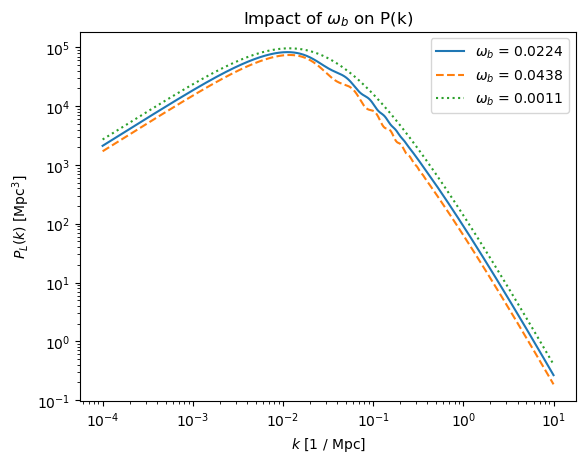
\includegraphics[scale=1.0]{intro/parameter_demos/ombh2_impact_on_Pk}
  \caption[Impact of $\omega_b$ on $P(k)$]{Impact of $\omega_b$. Increased
  	density in baryons corresponds to an increase in power on all scales.
  	However, this is not equivalent to a simple change in overall amplitude.
  	One counterexample is the shape of the BAO feature, which becomes more
  	pronounced for lower densities. A second counterexample is the location
  	of the turnover scale $k_s$, which is determined by the physical density
  	in baryons. However, this effect is subtle since the $x$-axis is
  	logarithmic and since even extreme values (relative to modern confidence
  	intervals) of $\omega_b$ will only slightly shift $k_s$. This shift
  	cannot be easily seen with the values used here.} 
  \label{fig: omega_b_dependence}
\end{figure}

\begin{figure}[htb]
  \centering
  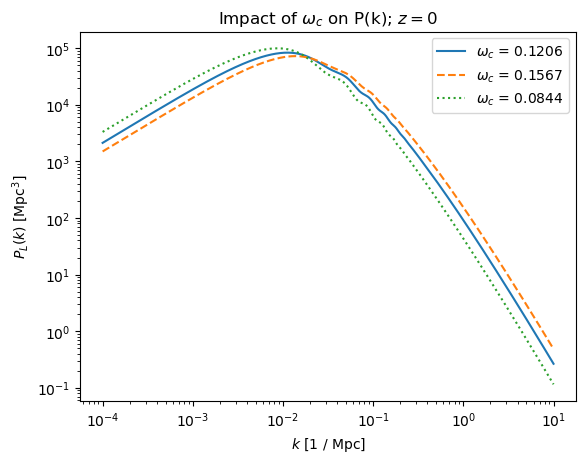
\includegraphics[scale=1.0]{intro/parameter_demos/omch2_impact_on_Pk}
  \caption[Impact of $\omega_c$ on $P(k)$]{Impact of $\omega_c$. Increased
  	density in CDM smooths out the BAO, similarly to the baryon case
  	(see figure~\ref{fig: omega_b_dependence}). More visibly, higher
  	densities shift power from larger to smaller scales due to gravitational 
  	collapse. Importantly, this behavior cannot be seen in the other
  	gravitationally interacting species, the baryons
  	(figure~\ref{fig: omega_b_dependence}). This is because, for all three
  	values used here for $\omega_c$ and for all three values used in
  	figure~\ref{fig: omega_b_dependence} for $\omega_b$,
  	$\omega_c > \omega_b$. This means that the baryon distribution will
  	largely be determined by the dynamics of CDM, rather than the
  	other way around. The dominant gravitationally-interacting species will
  	control the gravitational transfer of power from large to small scales.}
  \label{fig: omega_c_dependence}
\end{figure}

% If the gravitational collapse story were really true, why wouldn't that
% also apply to baryons? Maybe it's because b is so outnumbered by c

\begin{figure}[htb]
  \centering
  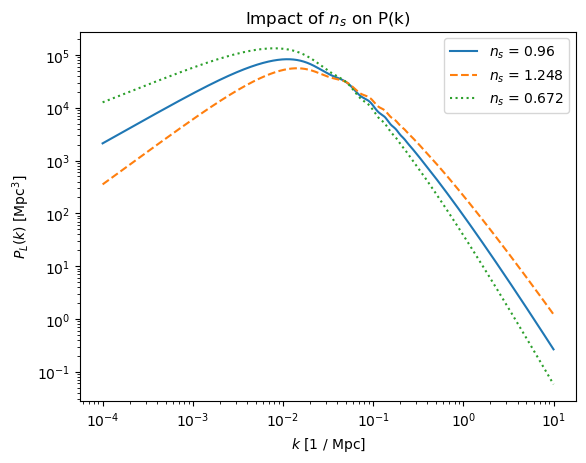
\includegraphics[scale=1.0]{intro/parameter_demos/n_s_impact_on_Pk}
  \caption[Impact of $n_s$ on $P(k)$]{Impact of $n_s$. The $n_s$ can be
  thought of as a kind of rotation of the power spectrum, although this
  is only coarse description. The differences shown here are
  adequately captured by equation~\ref{eq: n_s}.}
  \label{fig: n_s_dependence}
\end{figure}

\begin{figure}[htb]
  \centering
  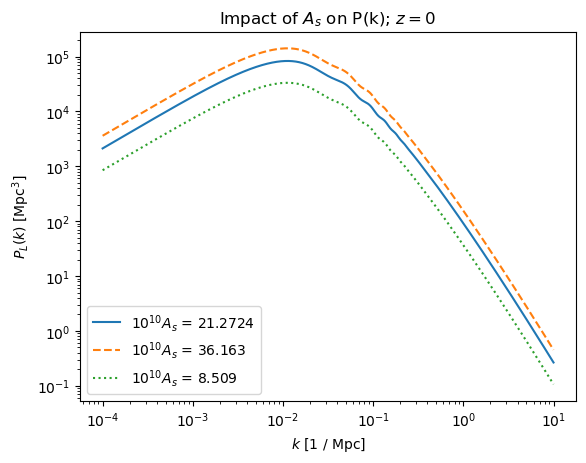
\includegraphics[scale=1.0]{intro/parameter_demos/A_s_impact_on_Pk}
  \caption[Impact of $A_s$ on $P(k)$]{Impact of $A_s$. Differences produce
  	only a change in the overall amplitude of the power spectrum. We stress
  	that this simple description applies only in the case of massless
  	neutrinos. The more subtle impact of $A_s$ will be demonstrated in
  	chapter~\ref{chap: A_s}. In the massless case, $A_s$ is completely
  	degenerate with $h$ (see figure~\ref{fig: without_h_units}) and with
  	$\sigma_{12}$ (not shown). This degeneracy is central to evolution
  	mapping, which will be discussed in section~\ref{sec: ev_mapping_intro}.}
  \label{fig: A_s_dependence}
\end{figure}

\begin{figure}[htb]
  \centering
  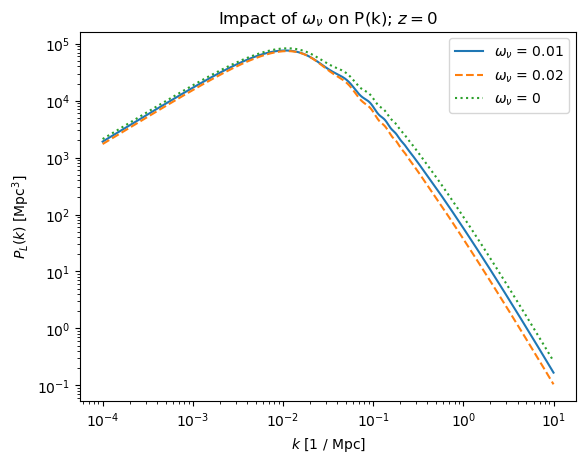
\includegraphics[scale=1.0]{intro/parameter_demos/omnuh2_impact_on_Pk}
  \caption[Impact of $\omega_\nu$ on $P(k)$]{Impact of $\omega_\nu$ for the
  	fixed redshift $z=0$. Massive neutrinos suppress structure formation in
  	a manner highly reminiscent of radiation. This similarity arises from the
  	combination of neutrinos' large velocities with the weakness of their 
  	interaction with other particles.
  	For the other primary parameters of this work,
  	the impact on power spectrum is independent of the value of $z$. This is
  	not the case with massive neutrinos
  	(see figure~\ref{fig: neutrinos_and_redshift}), which we will discuss in
  	section~\ref{sec: neutrino_problem}.}
  \label{fig: omega_nu_dependence}
\end{figure}

%s Segue into the next section

Since many of these parameters have fairly unique impacts on the power 
spectrum, we can imagine building a collection of power spectra labeled by
their parameter configurations and then comparing our real-world observations 
to them. We can ask to which of these theoretical power spectra our 
observations most closely agree. This question is quantitatively answered by 
parameter inference in the form of a Monte Carlo Markov Chain (MCMC) analysis, whose basic idea will be discussed in the next section.

%%% We're sinking this section! It's not relevant enough and I don't know 
%%% enough.
\begin{comment}

\section{Monte Carlo Markov Chains}

%Bayes' theorem states that

%\begin{equation}
%P(\bm{\pi} | \bm{d}) 
%\end{equation}

%We can assign a probability $P(\bm{\pi} | d$

This can be a very brief section, but I want to discuss a little bit of how most modern parameter inference works because it motivates the need for extremely fast power spectrum computation. It provides a sort of conceptual bridge between our ``pure'' goal (quantifying the cosmos) and the nitty-gritty bulk of the paper (optimizing emulator performance).

Metropolis-Hastings algorithm.

We don't know what the true probability distribution of power spectra is. In order to build this distribution with simulation results, we simply draw from the distribution. \textcolor{orange}{Refer to ``Data to Insights'' lecture notes in order to tighten this description.}

\end{comment}
%%%

\section{Evolution Mapping}
\label{sec: ev_mapping_intro}

\textcolor{blue}{I want to briefly summarize why we can funnel all of the 
evolution parameters through $\sigma_{12}$ in this way. This objective may be
too ambitious for this paper, because I would have to go through each
evolution parameter and derive its evolution nature in a few lines of 
equations.} \textcolor{orange}{Maybe I can just do the same thing as Ariel
recommended with the GPR kernel: ``we played around and found that this
works.''}

(\cbib{San21}) proposes to divide up the full set of cosmological
parameters into two categories: \textit{evolution} parameters $\mathcal{O}_E$
(such as $\omega_b$, $\omega_c$, and $\eta_s$)
affect the amplitude of the power spectrum at a particular redshift, while
\textit{shape} parameters $\mathcal{O}_S$
(such as $\omega_K$, $\omega_\text{DE}$, w(a))
affect the shape of the power
spectrum.

We take, as the evolution mapping relation for the power spectrum, equation 13
from \cbib{San21}:

\begin{equation}
\label{eq: evMapping_pSpectrum}
    \Delta^2_L (k | z, \Theta_s, \Theta_e)
    =
    \Delta_L^2 (k | \Theta_s, \sigma_{12} \left( z, \Theta_s, \Theta_e \right))
\end{equation}\footnote{Varying $z$ has the same effect as varying an
evolution parameter, which is why it appears on the RHS only as an argument to
the $\sigma_{12}$ ``function.'' We write it separately from $\Theta_e$ to
emphasize that $z$ does not describe a property of the Universe, but is
simply used as a proxy here for \textcolor{red}{conformal?} time
\textcolor{red}{elapsed since the Big Bang? (but we can only observe up to
$z = 1100$...)}.}

Why is this scheme important? Evolution mapping greatly simplifies the emulator
implementation. Because we can
funnel all of the evolution parameters through $\sigma_{12}$, we've effectively
collapsed an entire category of parameters to just one parameter. Fewer
parameters means that we get a more accurate emulator.

``At the linear level, all models characterized by identical shape parameters
and the same values of the parameter combinations $b \sigma_{12}(z)$ and
$f \sigma_{12}(z)$ will be identical'' (\cbib{San21}).

Now, for the hiccup, which segues into the next section: this scheme is broken by one parameter, the Universe's
density in neutrinos. (In the next section: why this is so and what we can do
about it.)

\section{Emulation: Basic Principles}
\label{sec: emulation_intro}

To conduct these MCMC analyses, we need several thousands of power spectra. However, if our Boltzmann solvers take on the order of three seconds to run, then these solvers will become the bottleneck of our analysis. \textcolor{orange}{Give some specific numbers for this.}

This motivates the introduction of emulation, basically multi-dimensional interpolation, in order to predict the power spectra. These predictions are orders of magnitude less time-expensive. 

Emulators interpolate across a high-dimensional parameter space. The primary
limitation is that the emulator has to be built with every possible parameter
in mind that an end-user could wish to vary. Yet there is a large number of
different cosmological parameters discussed in the modern literature.
``Currently available emulators only sample a few cosmological parameters,
often with restrictive ranges, and are not applicable to more general
parameter
spaces'' (\cbib{San21}). ``Due to the high computational cost of the required
simulations, [...] current emulators leave out parameters such as the
curvature
of the Universe or dynamic energy models beyond the standard CPL
parametrization'' (\cbib{San21}).

I'll talk a little about different emulators currently available, such as COMET. Some emulate non-linear power spectra, for example, and several even include massive neutrinos. But this thesis will demonstrate that massive neutrinos can be included into our evolution mapping approach, which will be introduced in section~\ref{sec: ev_mapping_intro}.

% (This is good news because the evolution mapping approach greatly simplifies the parameter space, and enhances the accuracy), which is the subject of the next section.

\section{Gaussian Process Regression}
\label{sec: gpr_intro}

% What is a Gaussian Process?

Most emulators are based on a Gaussian Process (GP). A GP is a Gaussian
distribution over functions\footnote
{A GP is the limit of a one-hidden-layer neural network as the number of
neurons approaches infinity.}, which can be interpreted
as the infinite-dimensional generalization of the multivariate normal
distribution. The inference of continuous values with a GP prior
is known as Gaussian process regression, or Kriging. GP regression is a
powerful non-linear multivariate interpolation tool. The computational
complexity of inference and likelihood evaluation within GP regression is cubic
in the number of points. This makes GP regression an excellent companion to
Latin hypercube sampling (LHS), which makes highly efficient use of a limited 
number of samples and whose basic idea will be explained in section~\ref{sec:
lhc_theory}.

Neural networks (NNs) generally need much larger sample sizes to reach
comparable levels of
accuracy. Due to various alterations in the Cassandra-Linear code over its
development, several regenerations of the various emulator data sets were
necessary. This practical constraint motivated the use of a GP for our
emulator. Furthermore, NNs invariably require much more complicated setup and
tuning--for example, in the precise architecture of the network (e.g. nodes
per layer, layer types) as well as the hyperparameters (e.g. learning rate).
By contrast, as we explain in section~\ref{sec: train_emu}, a Gaussian
process regression is highly straightforward to set up and modify. Therefore,
for a demonstration project such as Cassandra-Linear, we elected to base our
emulator on a GP. Please refer to the section~\ref{sec: future_work} for a
continuation of this discussion.

Are there other prediction approaches besides GPs and NNs? IF so, I need to
further justify WHY we’re using GPs.
GPs work best when there are few samples and a lot of parameters, right?
But why is that so? What is the math behind that?


\section{Sampling Approach: Latin Hypercube}
\label{sec: lhc_theory}

I imagine this is going to be an extremely short section. We should motivate why we're using this style of sampling.

What is the theoretical best LHC that we could make?

Besides, can we explain this equation?


\section{Neutrinos and Their Cosmological Impact}
\label{sec: neutrino_problem}

\begin{figure}[htb]
  \centering
  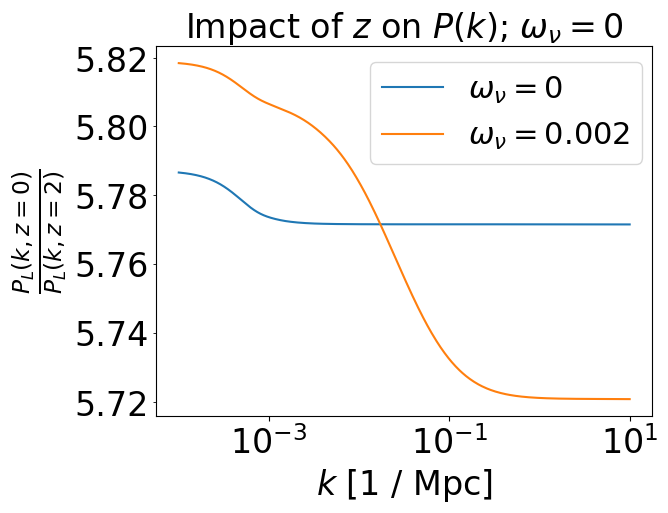
\includegraphics[scale=0.5]{intro/redshift_dependence_problem}
  \caption[Redshift Dependence of Neutrino Impact]{Blue is also not flat,
  	quite surprisingly.}
  \label{fig: neutrinos_and_redshift}
\end{figure}

(\cbib{Kiakotou}): ``Neutrinos with masses on the eV scale or below will be a
hot component of the dark matter and will free-stream out of overdensities and
thus wipe out small-scale structures.''

``In general, a larger density of relativistic species leads to a smaller
growth of matter fluctuations'' (\cbib{Zennaro}).

The point of this section is: why is $\omega_\nu$ bad for the
evolution mapping scheme? Because neutrinos exhibit redshift-dependent
damping of the power-spectrum, and therefore affect both the shape and the
amplitude of the power spectrum. Whenever massive neutrinos are present,
the growth factor becomes scale-dependent, which disrupts the
evolution-mapping scheme.

Why do they behave in this way? All neutrinos start off as
relativistic particles in the early Universe, acting as a type of radiation.
But as the Universe continues to expand and cool, the neutrinos behave
increasingly like dark matter.
In this way, the physical density in neutrinos impacts both the shape and the
evolution.

``The popular heuristic formula for the linear theory suppression of the matter
fluctuations by free-streaming $\nu$, $\Delta P(k) / P(k) \approx -8 f_\nu$, is
valid only on very small scales $k > 0.8 h$ / Mpc, However, it is not of
practical use as this is in the strongly nonlinear regime of matter
clustering'' (\cbib{Kiakotou}).

One proposed solution is to treat the neutrinos as a small correction factor
to the results from an anologous cosmology with the same $\omega_m$ but with
$\omega_\nu = 0$. This of course limits the applicability of our emulator to
cosmologies with very small $\omega_\nu$, but this constraint agrees with
current observations (\textcolor{orange}{which?}).

I want to end this section with a vague plan of action: we want to play around with CAMB power spectra to see if there are any simple ways around this limitation in our approach.

%%% New stuff

% what is a MEMNeC?

We already have an approximation for the power spectrum of a massive-neutrino cosmology within the evolution mapping scheme. The $\sigma_{12}$ value that we described earlier is actually the $\sigma_{12}$ value of the model's MEMNeC. can already be approximated within evolution-mapping by slightly altering scheme. \textcolor{red}{Is it fair to say we are adjusting, or was this actually the same scheme as it always was?} We take a MEMNeC and the desired cosmology. The sigma 12 is actually the sigma 12 of the MEMNeC. Then we treat the physical density in neutrinos as a shape parameter along with $A_s$.
